\chapter{الكمون الكهربائي؛ النواقل والمكثفات}\label{ch:b1:potential-capacitors}

المجال ثلاثة أعداد عند كل نقطة؛ والكمون عدد واحد. ولأن
القوة الكهرسكونية محافظة، يمكن طيّ مجال توزيع شحن كله
في دالة سلّمية واحدة، هي الكمون، ويُستعاد منها
بالاشتقاق --- وهو الاقتصاد نفسه الذي حوّل القوى إلى
\omterm{def:b1:work-and-energy:conservative}{طاقة كامنة} في الميكانيك. والكمون هو ما يقرؤه الفولطمتر، وما
يحفظه المولّد، وما يسرّع الإلكترونات في أنبوب؛ وأسطحه المتساوية
ترسم خريطة المجال بلمحة. ويبني هذا الفصل الكمون، ويستعمله
على ثنائي القطب (وهو أول نموذج كهربائي لجزيء)، ثم ينتقل إلى
الجسمين اللذين تُصنع منهما كل دارة: النواقل، التي تترتب الشحن
عليها بحيث تُميت المجال في الداخل، والمكثفات، التي تخزّن الشحنة والطاقة
في مجال.

\begin{omfigure}
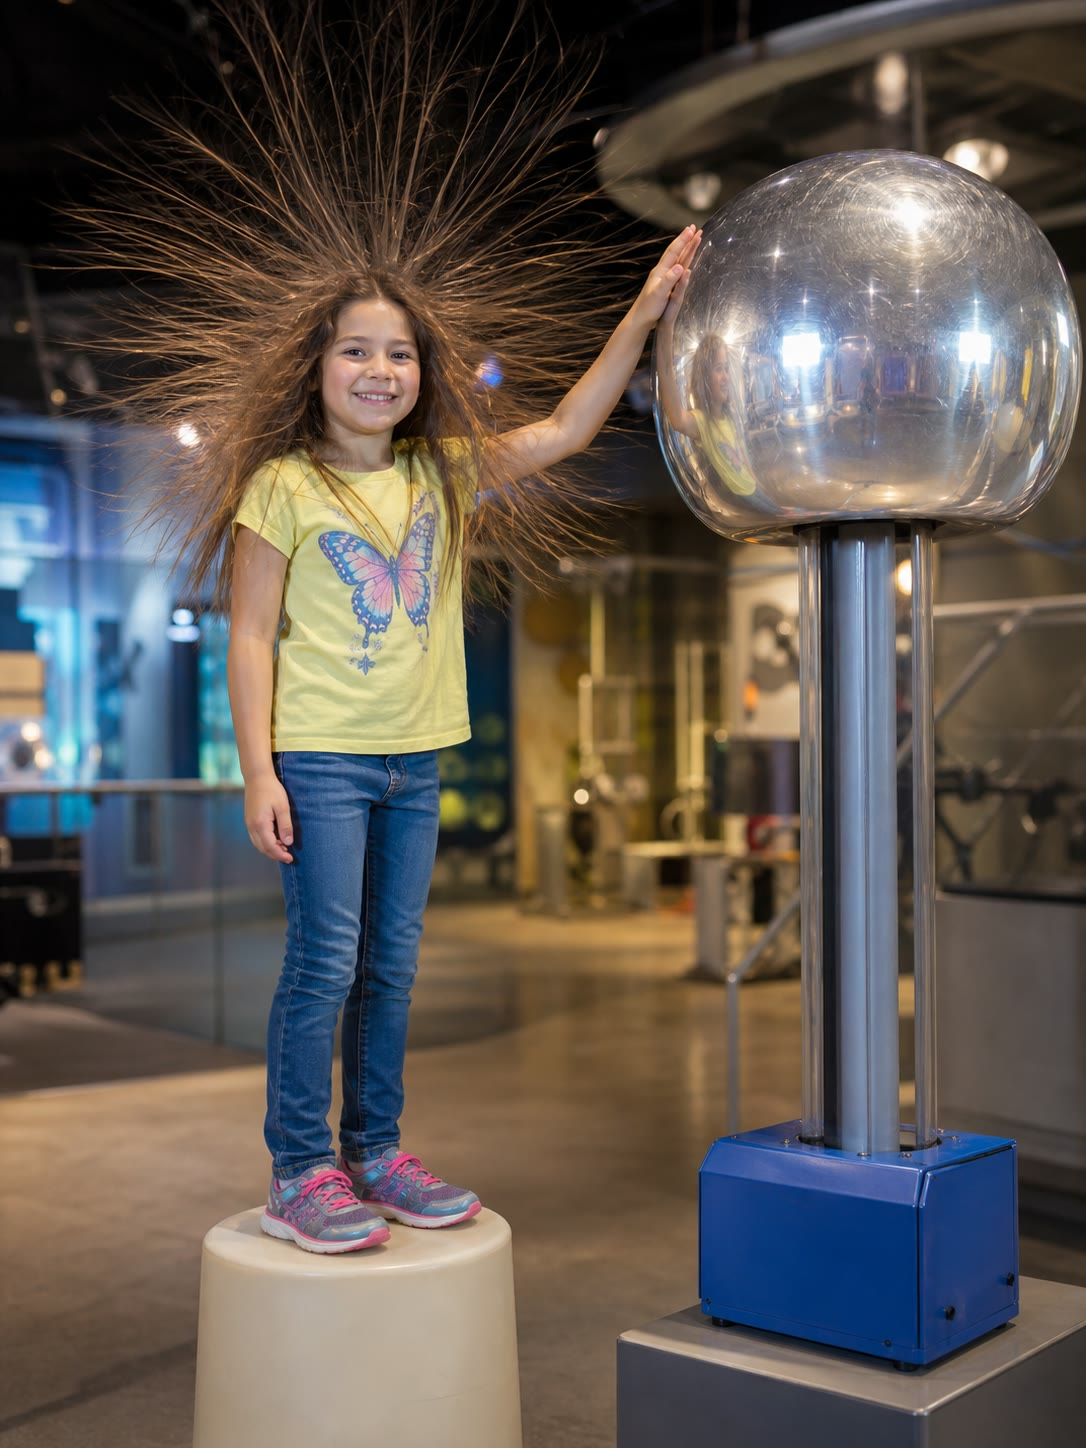
\includegraphics[width=0.34\linewidth]{images/book3/ai/b3-27-van-de-graaff-hair.jpg}

{\small شخص مشحون إلى بضع مئات من الكيلوفولطات بمولّد فان دي غراف: فهو ناقل متساوي الكمون تتنافر شعراته، وهي كلها عند الكمون نفسه ومشحونة الشحنة نفسها.}
\end{omfigure}

\section{الكمون الكهرسكوني}

\begin{theorem}[مجال الكهرباء الساكنة محافظ]\label{thm:b1:potential-capacitors:potential}
\index{كمون كهرسكوني}\index{فولط}\index{تكامل خطي}
توجد دالة سلّمية $V(M)$، هي \emph{\omterm{thm:b1:potential-capacitors:potential}{الكمون
الكهرسكوني}} (بالفولط، \unit{V})، بحيث يكون
\[
\vect E = -\overrightarrow{\operatorname{grad}}\,V , \qquad
V_A - V_B = \int_A^B \vect E\cdot\dd\vect l
\]
على امتداد أيّ مسار من $A$ إلى $B$ (فإن \emph{\omterm{thm:b1:potential-capacitors:potential}{التكامل الخطي}} للمتجهة $\vect E$
من $A$ إلى $B$ مستقل عن المسار، ومعدوم على امتداد حلقة
مغلقة). ومن أجل شحنة نقطية $q$ عند $O$ يكون $V(M) = \dfrac{q}{4\pi\varepsilon_0\,OM}$
مع الاصطلاح $V(\infty) = 0$؛ ومن أجل عدة شحن تتجمع
الكمونات. وطاقة الوضع لشحنة $q'$ عند $M$ هي $E_p = q'V(M)$، ويكون
شغل القوة الكهربائية من $A$ إلى $B$ هو $q'(V_A - V_B)$.
\end{theorem}

\begin{proof}
لقوة كولوم التي تؤثر بها شحنة ثابتة $q$ في $q'$ شكل
ثقالة نيوتن حيث يحلّ $-Gm_1m_2$ محلَّه المقدارُ $qq'/4\pi\varepsilon_0$؛ والحساب
نفسه الذي أعطى $E_p = -Gm_1m_2/r$
(\cref{prop:b1:work-and-energy:eps}) يعطي $E_p = qq'/4\pi\varepsilon_0r$:
وبالقسمة على $q'$ نجد $V$، ويكون $\vect E = \vect F/q' =
-\overrightarrow{\operatorname{grad}}(E_p)/q'$. ويحمل التراكب
النتيجة إلى أيّ توزيع؛ وصيغة \omterm{thm:b1:potential-capacitors:potential}{التكامل الخطي} هي تعريف
التدرج مكاملًا على امتداد المسار.
\end{proof}

\begin{proposition}[قراءة كمون]\label{prop:b1:potential-capacitors:reading}
\index{سطح متساوي الكمون}
\begin{enumerate}
  \item \emph{الأسطح المتساوية الكمون} $V = \text{ثابت}$ عمودية
        في كل موضع على \omterm{def:b1:electrostatics-gauss:field}{خطوط المجال}، ويتجه المجال نحو
        الكمون \emph{المتناقص}.
  \item $|\vect E|$ هو معدل تغيّر $V$ على امتداد الجهة
        الأشدّ ميلًا: فحيث تتقارب الأسطح المتساوية الكمون يكون المجال قويًّا.
  \item $V$ معرَّف إلى ثابت جمعي؛ ولا تُقاس إلا الفروق
        (أي التوترات). ويُجعل المرجع الأرضي أو اللانهاية معدومًا
        اصطلاحًا.
  \item في \omterm{def:b1:point-kinematics:spherical}{الإحداثيات الكروية} مع تناظر حول $O$ يكون $E_r = -\dd V/
        \dd r$؛ وفي \omterm{def:b1:point-kinematics:cylindrical}{الإحداثيات القطبية} $(r, \theta)$ في مستوٍ يكون
        $E_r = -\partial V/\partial r$ و $E_\theta = -\dfrac1r\,\partial V/\partial\theta$.
\end{enumerate}
\end{proposition}

\begin{proof}
على \omterm{prop:b1:potential-capacitors:reading}{سطح متساوي الكمون} يكون $\dd V = -\vect E\cdot\dd\vect l = 0$ من أجل كل
انزياح في السطح، فيكون $\vect E$ ناظميًّا عليه؛ وبالتحرك على امتداد
$\vect E$ يكون $\dd V = -E\,\dd l < 0$. وتأتي المركّبتان القطبيتان من
$\dd V = (\partial V/\partial r)\dd r + (\partial V/\partial\theta)\dd\theta$ ومن
$\dd\vect l = \dd r\,\vect e_r + r\,\dd\theta\,\vect e_\theta$.
\end{proof}

\begin{omfigure}
\begin{tikzpicture}[font=\small, x=1cm, y=1cm, >=Stealth]
  \begin{scope}
    \foreach \r in {0.6,0.85,1.2,1.7,2.4} \draw[omProp, thick] (0,0) circle (\r);
    \foreach \a in {0,30,...,330} \draw[omDef, ->] (0.25,0) ++({\a}:0) -- ++({\a}:2.7) ;
    \fill[omThm] (0,0) circle (2.5pt) node[below left, font=\footnotesize] {$q > 0$};
    \node[omProp, font=\footnotesize] at (2.05,2.05) {$V = \text{ثابت}$};
    \node[font=\footnotesize] at (0,-3.1) {شحنة نقطية: كرات $V \propto 1/r$};
  \end{scope}
  \begin{scope}[xshift=8.4cm]
    \draw[omThm, very thick] (-2.2,-2.2) -- (-2.2,2.2) node[above] {$V_1$};
    \draw[omDef, very thick] (2.2,-2.2) -- (2.2,2.2) node[above] {$V_2 < V_1$};
    \foreach \x in {-1.32,-0.44,0.44,1.32} \draw[omProp, thick] (\x,-2.0) -- (\x,2.0);
    \foreach \y in {-1.5,-0.5,0.5,1.5} \draw[omDef, ->] (-2.1,\y) -- (2.0,\y);
    \node[omProp, font=\footnotesize, anchor=west] at (-1.3,2.25) {أسطح متساوية الكمون};
    \node[font=\footnotesize] at (0,-3.1) {مكثف مستوٍ: مستويات، و $V$ خطي في $x$};
  \end{scope}
\end{tikzpicture}

{\small الأسطح المتساوية الكمون (بالبرتقالي) \omterm{def:b1:electrostatics-gauss:field}{وخطوط المجال} (بالأزرق) لشحنة
نقطية ولمكثف مستوٍ. وتقطع الخطوط الأسطحَ المتساوية الكمون
بزوايا قائمة وتجري من الكمون العالي إلى المنخفض؛ وحيث
تتزاحم تلك الأسطح يكون المجال قويًّا.}
\end{omfigure}

\begin{method}[حساب كمون]\label{meth:b1:potential-capacitors:compute}
إما أن تجمع $\dd q/4\pi\varepsilon_0r$ على التوزيع (حين يكون المجموع
قابلًا للحساب ويكون التوزيع منتهيًا، فيكون $V(\infty) = 0$ ذا
معنًى)، وإما أن تكامل $\dd V = -\vect E\cdot\dd\vect l$ على امتداد مسار ملائم
انطلاقًا من نقطة يُعرَف عندها $V$، مستعملًا المجال الذي يعطيه \omterm{thm:b1:electrostatics-gauss:gauss}{قانون
غاوس}. أما التوزيعات اللانهائية (سلك، مستوٍ) فلا تنفع فيها إلا الطريقة الثانية،
ويجب اختيار مبدأ $V$ عند نقطة منتهية.
\end{method}

\begin{proposition}[كمونات التوزيعات الكلاسيكية]\label{prop:b1:potential-capacitors:classic}
\begin{enumerate}
  \item كرة نصف قطرها $R$ وشحنتها $Q$ في حجمها: $V(r) = \dfrac{Q}{4\pi\varepsilon_0r}$
        في الخارج؛ و $V(r) = \dfrac{Q}{4\pi\varepsilon_0}\,\dfrac{3R^2 - r^2}{2R^3}$
        في الداخل، ومنه $V(0) = \tfrac32\,Q/4\pi\varepsilon_0R$. وإذا كانت $Q$ على السطح
        كان $V$ منتظمًا في الداخل ومساويًا $Q/4\pi\varepsilon_0R$.
  \item سلك لانهائي شحنته $\lambda$: $V(r) = -\dfrac{\lambda}{2\pi\varepsilon_0}\ln\dfrac{r}{r_0}$.
  \item \omterm{prop:b1:potential-capacitors:three}{مكثف مستوٍ}، مجاله $E$ من الصفيحة~1 إلى الصفيحة~2 على بعد $d$
        منها: يتناقص $V$ خطيًّا عبر الفجوة ويكون $V_1 - V_2 = Ed$.
\end{enumerate}
\end{proposition}

\begin{proof}
كامل $E_r = -\dd V/\dd r$ بمجالات
\cref{prop:b1:electrostatics-gauss:three}، من اللانهاية نحو الداخل في
الكرة (والاتصال عند $R$ يعيّن ثابت الداخل)، ومن $r_0$ في
السلك، وعبر الفجوة في \omterm{def:b1:potential-capacitors:capacitance}{المكثف}.
\end{proof}

\begin{omfigure}
\begin{tikzpicture}
\begin{axis}[omaxis, axis x line=bottom, axis y line=left, width=10cm, height=5.8cm,
    xlabel={$r/R$}, ylabel={},
    xlabel style={at={(axis description cs:0.5,-0.1)}, anchor=north},
    xmin=0, xmax=4, ymin=0, ymax=1.7, xtick={1,2,3}, ytick={0.5,1,1.5}, samples=80, clip=false]
  \addplot[omProp, very thick, domain=0:1] {1.5-0.5*x^2};
  \addplot[omProp, very thick, domain=1:4] {1/x};
  \node[omProp, font=\footnotesize, anchor=east] at (axis cs:3.95,1.5) {$V$ (بوحدات $Q/4\pi\varepsilon_0R$)};
  \addplot[omDef, thick, dashed, domain=0:1] {x};
  \addplot[omDef, thick, dashed, domain=1:4] {1/x^2};
  \node[omDef, font=\footnotesize, anchor=east] at (axis cs:3.95,1.27) {$E$ (بوحدات $Q/4\pi\varepsilon_0R^2$)};
  \node[omProp, font=\footnotesize, anchor=west] at (axis cs:0.05,1.58) {$V(0) = \tfrac32\,V(R)$};
\end{axis}
\end{tikzpicture}

{\small الكمون (بالخط المتصل) والمجال (بالمتقطع) لكرة مشحونة
بانتظام. فالكمون متصل وميله متصل؛ وهو
قطع مكافئ في الداخل، حيث يكون المجال خطيًّا، وبالمقدار $1/r$ في الخارج. ويقع
أعظميه عند المركز، حيث ينعدم المجال --- فأعظمي
$V$ نقطة مجال معدوم، لا العكس.}
\end{omfigure}

\begin{example}[الإلكترون-فولط من جديد]\label{ex:b1:potential-capacitors:eV}
إلكترون يعبر فجوة قدرها \qty{100}{V} يكسب $eU = \qty{100}{eV} =
\qty{1.6e-17}{J}$، مهما يكن شكل المجال بين
المسريين: فالكمون يجعل المسار بلا أهمية
(\cref{def:b1:charged-particles:eV}). وشحنة \qty{1}{\micro C} على بعد
\qty{1}{m} من أخرى لها $V = \qty{9}{kV}$ ويخزّن الزوج
\qty{9}{mJ}؛ والكمون في مركز نواة ذهب
\qty{24}{MV} (\cref{exo:b1:potential-capacitors:6}).
\end{example}

\section{ثنائي القطب الكهربائي}

\begin{definition}[ثنائي القطب الكهربائي]\label{def:b1:potential-capacitors:dipole}
\index{ثنائي قطب كهربائي}\index{عزم ثنائي القطب}
شحنتان متعاكستان $-q$ عند $N$ و $+q$ عند $P$، تفترقان بالمسافة $a = NP$،
تؤلفان \emph{ثنائي قطب كهربائيًّا} \emph{عزمه}
$\vect p = q\,\vect{NP}$ (بوحدة \unit{C.m})، متجهًا من $-$ إلى $+$. وتقريب
ثنائي القطب هو دراسة مجاله على مسافات $r \gg a$. وكل
جزيء لا ينطبق فيه مركز الشحنة الموجبة على مركز السالبة
(كالماء، $p = \qty{6.2e-30}{C.m}$) ثنائي قطب؛ والذرة المتعادلة في مجال
تصير كذلك (وهو ثنائي قطب مستحث).
\end{definition}

\begin{proposition}[مجال ثنائي القطب]\label{prop:b1:potential-capacitors:dipolefield}
عند $M$ مع $OM = r \gg a$ (حيث $O$ منتصف $NP$) و $\theta$
الزاوية بين $\vect p$ و $\vect{OM}$، يكون
\[
V(M) = \frac{p\cos\theta}{4\pi\varepsilon_0 r^2}, \qquad
E_r = \frac{2p\cos\theta}{4\pi\varepsilon_0r^3}, \qquad
E_\theta = \frac{p\sin\theta}{4\pi\varepsilon_0r^3} .
\]
ويتناقص مجال ثنائي القطب بنسبة $1/r^3$، أسرع من $1/r^2$
للشحنة: فمن بعيد تكاد الشحنتان تتلاشيان، ولا يبقى إلا
تباعدهما.
\end{proposition}

\begin{proof}
$V = \dfrac{q}{4\pi\varepsilon_0}\Bigl(\dfrac1{PM} - \dfrac1{NM}\Bigr)$ مع
$PM \approx r - \tfrac a2\cos\theta$ و $NM \approx r + \tfrac a2\cos\theta$
(بإسقاط $\pm\tfrac a2$ على $\vect{OM}$)؛ وإلى المرتبة الأولى في $a/r$ يكون
$1/PM - 1/NM \approx a\cos\theta/r^2$. ثم $E_r = -\partial V/\partial r$ و
$E_\theta = -(1/r)\,\partial V/\partial\theta$.
\end{proof}

\begin{omfigure}
\begin{tikzpicture}[font=\small, x=1cm, y=1cm, >=Stealth]
  \begin{scope}[scale=1.3]
    \fill[omDef] (-0.5,0) circle (2.5pt) node[below left, font=\footnotesize] {$-q$};
    \fill[omThm] (0.5,0) circle (2.5pt) node[below right, font=\footnotesize] {$+q$};
    \draw[->, very thick] (-0.5,0) -- (0.5,0); \node[above, font=\footnotesize] at (0,0.05) {$\vect p$};
    \fill (0,0) circle (1pt); \node[below, font=\footnotesize] at (0,-0.05) {$O$};
    \coordinate (M) at (2.6,1.9);
    \fill (M) circle (1.6pt) node[above right, font=\footnotesize] {$M$};
    \draw[dashed] (0,0) -- (M) node[midway, above left, font=\footnotesize] {$r$};
    \draw[dashed] (-0.5,0) -- (M); \draw[dashed] (0.5,0) -- (M);
    \draw (0.9,0) arc[start angle=0, end angle=36, radius=0.9] node[midway, right, font=\footnotesize] {$\theta$};
    \draw[->, omThm, thick] (M) -- ++(36:0.9) node[right, font=\footnotesize] {$E_r$};
    \draw[->, omThm, thick] (M) -- ++(126:0.6) node[above left, font=\footnotesize] {$E_\theta$};
  \end{scope}
  \begin{scope}[xshift=8.6cm, scale=1.0]
    % field lines: circles through the charges (dipole limit: r = K sin^2 theta)
    \foreach \K in {0.8,1.6,2.6} {
      \draw[omDef, thick, domain=3:177, samples=60, smooth] plot ({\K*sin(\x)*sin(\x)*cos(\x)}, {\K*sin(\x)*sin(\x)*sin(\x)});
      \draw[omDef, thick, domain=183:357, samples=60, smooth] plot ({\K*sin(\x)*sin(\x)*cos(\x)}, {\K*sin(\x)*sin(\x)*sin(\x)});
    }
    % equipotentials r = A sqrt(|cos theta|)
    \foreach \A in {0.9,1.5,2.2} {
      \draw[omProp, thick, domain=-88:88, samples=50, smooth] plot ({\A*sqrt(cos(\x))*cos(\x)}, {\A*sqrt(cos(\x))*sin(\x)});
      \draw[omProp, thick, domain=92:268, samples=50, smooth] plot ({\A*sqrt(-cos(\x))*cos(\x)}, {\A*sqrt(-cos(\x))*sin(\x)});
    }
    \draw[->, very thick] (-0.25,0) -- (0.25,0);
    \node[font=\footnotesize, omProp] at (2.95,0.45) {$V > 0$};
    \node[font=\footnotesize, omProp] at (-2.95,0.45) {$V < 0$};
  \end{scope}
\end{tikzpicture}

{\small على اليمين: هندسة تقريب ثنائي القطب --- فالنقطة $M$ منظورًا إليها من
المركز $O$ على البعد $r$ وبالزاوية $\theta$ عن $\vect p$، مع
مركّبتَي المجال القطرية والمعامدة. وعلى اليسار: \omterm{def:b1:electrostatics-gauss:field}{خطوط المجال} (بالأزرق،
$r \propto \sin^2\theta$) والأسطح المتساوية الكمون (بالبرتقالي، $r \propto
\sqrt{|\cos\theta|}$) لثنائي قطب متجه إلى اليمين؛ والمستوي المارّ بالنقطة $O$
والعمودي على $\vect p$ هو \omterm{prop:b1:potential-capacitors:reading}{السطح المتساوي الكمون} $V = 0$.}
\end{omfigure}

\begin{proposition}[ثنائي قطب في مجال خارجي]\label{prop:b1:potential-capacitors:dipoleinfield}
\index{ثنائي قطب!العزم المزدوج}\index{ثنائي قطب!الطاقة}
ثنائي قطب $\vect p$ في مجال منتظم $\vect E$ لا يحسّ بأيّ قوة صافية، بل
بعزم مزدوج $\vect\Gamma = \vect p\wedge\vect E$ ينحو إلى مطابقته مع
المجال، وتكون له طاقة الوضع $E_p = -\vect p\cdot\vect E$،
وهي أصغرية عند المطابقة. وفي مجال غير منتظم يُجذب فوق ذلك
نحو مناطق المجال القوي (وفي بعد واحد $F_x = p\,\dd E/\dd x$
من أجل ثنائي قطب مطابق).
\end{proposition}

\begin{proof}
القوتان $\pm q\vect E$ تتلاشيان؛ وعزمهما بالنسبة إلى $O$ هو $\vect{OP}\wedge
q\vect E + \vect{ON}\wedge(-q\vect E) = q\vect{NP}\wedge\vect E$. وأما الطاقة:
$qV(P) - qV(N) = -q\,\vect{NP}\cdot\vect E$ في مجال منتظم (لأن $V(P)
- V(N) = -\vect E\cdot\vect{NP}$). وفي مجال غير منتظم، مع مطابقة على امتداد $x$: $F_x =
qE(x + a) - qE(x) \approx qa\,\dd E/\dd x$.
\end{proof}

\begin{example}[لماذا يجذب المشط الورق]\label{ex:b1:potential-capacitors:comb}
يُحدث مشط مشحون مجالًا يتناقص مع البعد؛ وقصاصة من
الورق، وهي متعادلة، تستقطبها (فتصير ثنائي قطب مستحثًّا على امتداد $\vect E$)،
وتجذبها القوة $p\,\dd E/\dd x$ على ثنائي قطب مطابق نحو
منطقة المجال القوي: أي نحو المشط. ولا أهمية لإشارة شحنة المشط؛
والآلية نفسها تُبقي المنطاد على الجدار وتجعل
خيط الماء ينحرف. وفي جزيئات الماء يكون $pE$ في مجال \qty{1}{MV/m}
مساويًا \qty{6e-24}{J}، أي أصغر $600$ مرة من $k_BT$ عند \omterm{def:b1:kinetic-theory:temperature}{درجة حرارة} الغرفة:
فلا تنجو من التقلّب الحراري إلا مطابقة صافية طفيفة
(\cref{exo:b1:potential-capacitors:7}).
\end{example}

\section{النواقل في التوازن الكهرسكوني}

\begin{theorem}[خواصّ ناقل في التوازن]\label{thm:b1:potential-capacitors:conductor}
\index{ناقل في التوازن}\index{مبرهنة كولوم}\index{قفص فاراداي}
في ناقل تكون فيه الشحن الحرة ساكنة:
\begin{enumerate}
  \item $\vect E = \vect 0$ في الداخل، ويكون الناقل حجمًا متساوي
        الكمون: فيكون $V$ منتظمًا فيه وعلى سطحه.
  \item تستقر أيّ شحنة صافية على السطح، بكثافة سطحية
        $\sigma$؛ ويكون الداخل متعادلًا.
  \item وفي الخارج مباشرةً يكون المجال ناظميًّا على السطح ومساويًا
        $\vect E = \dfrac{\sigma}{\varepsilon_0}\,\vect n$ (وهي \emph{\omterm{thm:b1:potential-capacitors:conductor}{مبرهنة كولوم}}).
  \item وفي تجويف داخل ناقل، خالٍ من الشحنة، يكون $\vect E =
        \vect 0$ و $V$ منتظمًا مهما يجرِ في الخارج (وهو \emph{\omterm{thm:b1:potential-capacitors:conductor}{قفص
        فاراداي}}).
\end{enumerate}
\end{theorem}

\begin{proof}
(1) كان مجالٌ ليحرّك الشحن الحرة: فيقتضي التوازن $\vect E =
\vect 0$، ومنه $\dd V = 0$ بين أيّ نقطتين داخليتين؛ والسطح
هو النهاية. (2) \omterm{thm:b1:electrostatics-gauss:gauss}{قانون غاوس} على أيّ سطح مغلق يُرسم داخل
الناقل: تدفق معدوم، فشحنة محصورة معدومة. (3) \omterm{prop:b1:potential-capacitors:reading}{والسطح
متساوي الكمون}، فيكون $\vect E$ في الخارج مباشرةً ناظميًّا عليه؛ ولعلبة مسطّحة
تعتلي السطح تدفقٌ $E\,\dd S$ عبر وجهها الخارجي وحده
(إذ $\vect E = \vect 0$ في الداخل) وشحنةٌ $\sigma\,\dd S$. (4) وجدار التجويف
متساوي الكمون؛ وكان خط مجال داخل التجويف ليضطر إلى
الذهاب من الجدار إلى الجدار عبر هبوط في الكمون --- وهو مستحيل على
\omterm{prop:b1:potential-capacitors:reading}{سطح متساوي الكمون}؛ فلا خط ولا مجال (مسلَّم به بهذه الصيغة).
\end{proof}

\begin{example}[أثر الأطراف ومانعة الصواعق]\label{ex:b1:potential-capacitors:point}
\index{أثر الأطراف}
كرتان نصفا قطريهما $R_1 > R_2$، متباعدتان وموصولتان بسلك، لهما
$V = Q_i/4\pi\varepsilon_0R_i$ نفسه، ومنه $\sigma_i = Q_i/4\pi R_i^2 = \varepsilon_0V/R_i$:
فكلما \emph{صغر} نصف قطر الانحناء \emph{كبرت} الشحنة
السطحية والمجال $\sigma/\varepsilon_0 = V/R$. وعند طرف مدبَّب يتجاوز المجال
قيمة انهيار الهواء (\qty{3}{MV/m}) قبل أن يتجاوزها في
أيّ موضع آخر بكثير: فيتأيّن الهواء وتتسرب الشحنة بهدوء. وتعمل
مانعة الصواعق بما يسمّى \emph{\omterm{ex:b1:potential-capacitors:point}{أثر الأطراف}} --- فهي لا تجذب
الضربة بقدر ما تعرض عليها مسلكًا، وتنزف الشحنة تحت
سحابة قبل أن تتراكم.
\end{example}

\begin{omfigure}
\begin{tikzpicture}[font=\small, x=1cm, y=1cm, >=Stealth]
  % Faraday cage
  \begin{scope}
    \draw[fill=omExo!20, draw=omExo, thick] (-1.6,-1.3) rectangle (1.6,1.3);
    \draw[fill=white, draw=omExo, thick] (-1.0,-0.75) rectangle (1.0,0.75);
    \foreach \y in {-1.0,-0.5,0,0.5,1.0} \draw[omDef, ->] (-3.0,\y) -- (-1.65,\y);
    \foreach \y in {-1.0,-0.5,0,0.5,1.0} \draw[omDef, ->] (1.65,\y) -- (3.0,\y);
    \foreach \y in {-1.0,-0.5,0,0.5,1.0} {\node[omDef, font=\scriptsize] at (-1.75,\y+0.18) {$-$}; \node[omThm, font=\scriptsize] at (1.75,\y+0.18) {$+$};}
    \node[font=\footnotesize] at (0,0) {$\vect E = \vect 0$};
    \node[font=\footnotesize] at (0,-1.85) {ناقل في مجال خارجي};
  \end{scope}
  % point effect
  \begin{scope}[xshift=8.4cm]
    \draw[fill=omExo!20, draw=omExo, thick] (-1.2,0) circle (1.2);
    \draw[fill=omExo!20, draw=omExo, thick] (0,0.12) -- (2.4,0.0) -- (0,-0.12) -- cycle;
    \draw[omExo, thick] (2.4,0) circle (0.06);
    \foreach \a in {100,135,170,205,240,275} \draw[omDef, ->] (-1.2,0) ++({\a}:1.25) -- ++({\a}:0.5);
    \foreach \a in {-40,-20,0,20,40} \draw[omDef, ->] (2.4,0) ++({\a}:0.1) -- ++({\a}:1.2);
    \node[font=\footnotesize, omDef] at (-1.2,2.0) {$\sigma$ صغيرة، و $E$ ضعيف};
    \node[font=\footnotesize, omDef] at (2.6,1.0) {$\sigma$ كبيرة، و $E$ قوي};
    \node[font=\footnotesize] at (0.6,-1.85) {$V$ نفسه في كل موضع: المجال $\propto 1/R$};
  \end{scope}
\end{tikzpicture}

{\small على اليمين: ناقل مجوَّف في مجال خارجي --- فالشحن
المستحثة على سطحه تلاشي المجال في الداخل وفي التجويف (وهو
\omterm{thm:b1:potential-capacitors:conductor}{قفص فاراداي}). وعلى اليسار: \omterm{ex:b1:potential-capacitors:point}{أثر الأطراف} --- فعلى ناقل واحد متساوي الكمون
تكون الشحنة السطحية والمجال الخارجي أكبر ما يكونان حيث
يكون الانحناء أشدّ حدّة.}
\end{omfigure}

\section{المكثفات}

\begin{definition}[السعة]\label{def:b1:potential-capacitors:capacitance}
\index{سعة}\index{مكثف}\index{فاراد}
ناقل معزول عند الكمون $V$ يحمل شحنة $Q$
تتناسب مع $V$: $Q = CV$، حيث $C$ هي \emph{سعته} (بالفاراد،
\unit{F})؛ وللكرة $C = 4\pi\varepsilon_0R$. و\emph{المكثف} زوج
من النواقل (هما \emph{صفيحتاه}) يحملان شحنتين متعاكستين $\pm Q$
ويتقابلان بحيث يكون المجال محصورًا بينهما؛ وسعته
هي $C = Q/U$ حيث $U = V_1 - V_2$ التوتر بين
الصفيحتين. وقد استُعمل رمزه وقانون الدارة $i = C\,\dd u/\dd t$ في
\cref{ch:b1:transient-regimes}.
\end{definition}

\begin{proposition}[ثلاثة مكثفات]\label{prop:b1:potential-capacitors:three}
\index{مكثف مستوٍ}\index{مكثف كروي}\index{مكثف أسطواني}
\begin{enumerate}
  \item المستوي: صفيحتان مساحة كلٍّ منهما $S$ وتفترقان بالمسافة $d \ll \sqrt S$:
        $C = \dfrac{\varepsilon_0S}{d}$.
  \item الكروي: كرتان متحدتا المركز نصفا قطريهما $R_1 < R_2$:
        $C = \dfrac{4\pi\varepsilon_0R_1R_2}{R_2 - R_1}$.
  \item الأسطواني (المحوري)، نصفا القطرين $a < b$ والطول $L \gg b$:
        $C = \dfrac{2\pi\varepsilon_0L}{\ln(b/a)}$.
\end{enumerate}
وملء الفجوة بعازل سماحيته النسبية
$\varepsilon_r$ يضرب $C$ بالعامل $\varepsilon_r$ (إذ تستقطب جزيئات العازل
فتُضعف المجال، و $\varepsilon_r = 2$ إلى $10$ في اللدائن
والزجاج الشائعة، و $80$ في الماء).
\end{proposition}

\begin{proof}
في كل حالة يكون المجال بين الصفيحتين مجالَ
\cref{prop:b1:electrostatics-gauss:three}: فيكون $E = \sigma/\varepsilon_0 = Q/\varepsilon_0S$
و $U = Ed$؛ و $E = Q/4\pi\varepsilon_0r^2$ و $U = \int_{R_1}^{R_2}E\,\dd r = \dfrac{Q}{4\pi\varepsilon_0}
\Bigl(\dfrac1{R_1} - \dfrac1{R_2}\Bigr)$؛ و $E = Q/2\pi\varepsilon_0Lr$ و $U =
\dfrac{Q}{2\pi\varepsilon_0L}\ln\dfrac ba$. ثم اقسم $Q$ على $U$. أما عامل العازل
فمسلَّم به.
\end{proof}

\begin{theorem}[طاقة مكثف]\label{thm:b1:potential-capacitors:energy}
\index{طاقة مكثف}\index{كثافة طاقة المجال الكهربائي}
\omterm{def:b1:potential-capacitors:capacitance}{مكثف} مشحون إلى $Q$ تحت التوتر $U$ يخزّن
\[
W = \tfrac12 CU^2 = \tfrac12 QU = \frac{Q^2}{2C} ,
\]
وهو الشغل اللازم لنقل الشحنة من صفيحة إلى الأخرى
في مواجهة التوتر المتزايد. وفي \omterm{prop:b1:potential-capacitors:three}{مكثف مستوٍ} يكون $W = \tfrac12\varepsilon_0E^2
\times Sd$: فالطاقة في المجال، بكثافة $\tfrac12\varepsilon_0E^2$
لواحدة الحجم --- وهي عبارة تصحّ من أجل كل مجال
كهرسكوني.
\end{theorem}

\begin{proof}
نقل $\dd q$ من الصفيحة السالبة إلى الموجبة حين تكون الشحنة
$q$ يكلّف $\dd W = (q/C)\,\dd q$؛ فكامل من $0$ إلى $Q$. ثم
عوّض $C = \varepsilon_0S/d$ و $U = Ed$؛ أما الكثافة العامة فمسلَّم بها.
\end{proof}

\begin{example}[ثلاثة مكثفات وطاقاتها]\label{ex:b1:potential-capacitors:energies}
زوج من الرقائق مساحته متر مربع ويفترقان \qty{1}{mm}: $C = 8.85 \times 10^{-12}/
10^{-3} = \qty{8.9}{nF}$ --- \omterm{def:b1:potential-capacitors:capacitance}{فالفاراد} وحدة هائلة. \omterm{def:b1:potential-capacitors:capacitance}{ومكثف} مزيل رجفان
سعته \qty{150}{\micro F} عند \qty{2}{kV}: \qty{300}{J}، تُقدَّم في ميلي ثوانٍ.
\omterm{def:b1:potential-capacitors:capacitance}{ومكثف} فائق سعته \qty{3000}{F} عند \qty{2.7}{V}: \qty{11}{kJ} في علبة
بحجم قارورة مشروب --- وتأتي \omterm{def:b1:potential-capacitors:capacitance}{سعته} من فجوة
جزيئية $d$ ومن مساحة $S$ مسامية هائلة. وكثافة طاقة مجال عند
انهيار الهواء، $\tfrac12\varepsilon_0(3 \times 10^6)^2 = \qty{40}{J/m^3}$، هي
سبب أن المكثفات تخزّن قليلًا جدًّا بالقياس إلى البطاريات.
\end{example}

\begin{omfigure}
\begin{tikzpicture}[font=\small, x=1cm, y=1cm, >=Stealth]
  \begin{scope}
    \draw[omThm, very thick] (-1.5,1) -- (1.5,1) node[right, font=\footnotesize] {$+Q$, $V_1$};
    \draw[omDef, very thick] (-1.5,-1) -- (1.5,-1) node[right, font=\footnotesize] {$-Q$, $V_2$};
    \foreach \x in {-1.1,-0.55,0,0.55,1.1} \draw[omProp, ->] (\x,0.9) -- (\x,-0.85);
    \draw[omProp, dashed] (-1.55,0.9) .. controls (-2.2,0.5) and (-2.2,-0.5) .. (-1.55,-0.85);
    \draw[omProp, dashed] (1.55,0.9) .. controls (2.2,0.5) and (2.2,-0.5) .. (1.55,-0.85);
    \draw[<->] (-2.6,1) -- (-2.6,-1) node[midway, left, font=\footnotesize] {$d$};
    \node[font=\footnotesize] at (0,-1.7) {مستوٍ: $C = \varepsilon_0S/d$};
    \node[font=\footnotesize, omProp, fill=white, inner sep=1.5pt] at (0.27,0.3) {$E = U/d$};
  \end{scope}
  \begin{scope}[xshift=6.2cm]
    \draw[omDef, very thick] (0,0) circle (1.3);
    \draw[omThm, very thick, fill=omThm!15] (0,0) circle (0.55);
    \foreach \a in {0,60,...,300} \draw[omProp, ->] (0,0) ++({\a}:0.6) -- ++({\a}:0.6);
    \draw[<->] (0,0) -- (225:0.55) node[midway, above left, font=\scriptsize] {$R_1$};
    \draw[<->] (0,0) -- (-20:1.3) node[pos=0.75, below, font=\scriptsize] {$R_2$};
    \node[font=\footnotesize] at (0,-1.7) {كروي (أو أسطواني، بمقطع)};
  \end{scope}
  \begin{scope}[xshift=11.2cm]
    \fill[omExo!25] (-1.2,-0.95) rectangle (1.2,0.95);
    \draw[omThm, very thick] (-1.2,1) -- (1.2,1);
    \draw[omDef, very thick] (-1.2,-1) -- (1.2,-1);
    \node[font=\footnotesize] at (0,0) {$\varepsilon_r$};
    \node[font=\footnotesize] at (0,-1.7) {عازل: $C \to \varepsilon_rC$};
  \end{scope}
\end{tikzpicture}

{\small مكثفات مستوية وكروية ومملوءة بعازل. والمجال
(بالبرتقالي) محصور بين الصفيحتين إلا عند انتشاره على
الحواف، وهو ما يُهمَل حين يكون $d$ صغيرًا؛ وتعيش الطاقة $\tfrac12\varepsilon_0E^2$
لواحدة الحجم في ذلك المجال.}
\end{omfigure}

\begin{remark}[ربط المكثفات]\label{rem:b1:potential-capacitors:association}
على التفرع (بالتوتر $U$ نفسه) تتجمع الشحن: $C = C_1 + C_2$؛ وعلى التسلسل (بالشحنة
$Q$ نفسها) تتجمع التوترات: $1/C = 1/C_1 + 1/C_2$ --- وهو عكس
المقاومات، لأن $C$ تقيس سهولة (شحنة لكل فولط) حيث تقيس $R$
صعوبة. وتتبع هاتان القاعدتان من $Q = CU$ ومن
قوانين الدارات في \cref{ch:b1:dc-circuits}.
\end{remark}

\section{تمارين}

\begin{exercise}[$\star$]\label{exo:b1:potential-capacitors:1}
الكمون على بعد \qty{1.0}{m} من شحنة \qty{1.0}{\micro C}؛ والطاقة اللازمة
لجلب شحنة ثانية \qty{1.0}{\micro C} من اللانهاية إلى تلك النقطة؛ والسرعة
التي كانت لتنطلق بها لو أُطلقت، إن كانت كتلتها \qty{1}{g}.
\end{exercise}

\begin{exercise}[$\star$]\label{exo:b1:potential-capacitors:2}
صفيحتان تفترقان \qty{1.0}{mm} تحت \qty{100}{V}: أوجد المجال؛ \omterm{thm:b1:work-and-energy:ke}{والطاقة الحركية}
والسرعة اللتين يكسبهما إلكترون يعبر الفجوة من السكون؛ وزمن
الطيران.
\end{exercise}

\begin{exercise}[$\star$]\label{exo:b1:potential-capacitors:3}
على خريطة أسطح متساوية الكمون مرسومة كل \qty{10}{V}، تفترق الخطوط
\qty{2}{mm} قرب $A$ و\qty{8}{mm} قرب $B$. أوجد المجال عند $A$
وعند $B$؛ وإلى أيّ جهة يتجه المجال بالنسبة إلى الكمونات
المتزايدة؛ وإلى أيّ جهة يتسارع إلكترون؟
\end{exercise}

\begin{exercise}[$\star$]\label{exo:b1:potential-capacitors:4}
كرة فان دي غراف نصف قطرها \qty{15}{cm} تُشحن إلى \qty{200}{kV}.
أوجد \omterm{def:b1:potential-capacitors:capacitance}{السعة} والشحنة والمجال عند سطحها. وأكبر كمون قبل أن
ينهار الهواء من حولها (\qty{3}{MV/m}).
\end{exercise}

\begin{exercise}[$\star\star$]\label{exo:b1:potential-capacitors:5}
الكمون على محور حلقة نصف قطرها $R$ وشحنتها $Q$؛ ثم استعد
المجال المحوري بالاشتقاق. والسؤال نفسه من أجل القرص المشحون بانتظام
(باستعمال \cref{exo:b1:electrostatics-gauss:5}): $V(z) = \dfrac{\sigma}{2\varepsilon_0}
\bigl(\sqrt{z^2 + R^2} - z\bigr)$.
\end{exercise}

\begin{exercise}[$\star\star$]\label{exo:b1:potential-capacitors:6}
اشتقّ الكمون داخل كرة مشحونة بانتظام من مجالها.
وأوجد الكمون في مركز نواة ذهب ($Z = 79$ و $R = \qty{7.0}{fm}$)؛
والطاقة التي كان بروتون ليحتاج إليها ليبلغ المركز من بعيد،
بوحدة \unit{MeV}؛ وعلّق على جسيمات ألفا ذات \qty{5}{MeV} عند رذرفورد.
\end{exercise}

\begin{exercise}[$\star\star$]\label{exo:b1:potential-capacitors:7}
جزيء ماء، $p = \qty{6.2e-30}{C.m}$. أوجد المجال الذي يُحدثه على \qty{1.0}{nm}
على امتداد محوره وعموديًّا عليه؛ والعزم المزدوج وفرق الطاقة
بين الوضعين المطابق والمعاكس في $E = \qty{1.0}{MV/m}$؛
وقارن بالمقدار $k_BT$ عند \qty{300}{K}. ثم مجال أيون صوديوم عند
\qty{0.3}{nm} وطاقة ثنائي قطب الماء المطابق فيه (وهي الإماهة).
\end{exercise}

\begin{exercise}[$\star\star$]\label{exo:b1:potential-capacitors:8}
كرة ناقلة نصف قطرها \qty{1.0}{cm} في الهواء: أوجد أكبر شحنة
وأكبر كمون قبل الانهيار. وكرتان ناقلتان، $R_1 = \qty{10}{cm}$
و $R_2 = \qty{1.0}{mm}$، موصولتان بسلك رفيع ومرفوعتان إلى
\qty{20}{kV}: أوجد المجال السطحي على كلٍّ منهما؛ وأيّهما يفرّغ في الهواء؟
\end{exercise}

\begin{exercise}[$\star\star$]\label{exo:b1:potential-capacitors:9}
السعات: رقيقتان مساحة كلٍّ منهما \qty{1.0}{m^2} تفترقان \qty{10}{\micro m} مع
شريحة بوليمرية $\varepsilon_r = 2.2$ (وهو \omterm{def:b1:potential-capacitors:capacitance}{مكثف} شريحي)؛ والرقيقتان نفسهما ملفوفتان
--- فهل يغيّر اللفّ $C$؟ ثم الطاقة عند \qty{400}{V}. \omterm{def:b1:potential-capacitors:capacitance}{ومكثف} \qty{150}{\micro F}
عند \qty{2.0}{kV} (مزيل رجفان): أوجد الشحنة والطاقة ومتوسط الاستطاعة إن
قُدِّمت في \qty{5}{ms}.
\end{exercise}

\begin{exercise}[$\star\star\star$]\label{exo:b1:potential-capacitors:10}
\emph{المكثفان الكروي والأسطواني.} (أ) اشتقّ $C$ من أجل
كرتين متحدتَي المركز وتحقّق من أنه، حين $R_2 - R_1 = d \ll R_1$، يؤول
إلى صيغة المستوي، وحين $R_2 \to \infty$ إلى الكرة المعزولة.
(ب) كبل محوري، $a = \qty{0.5}{mm}$ و $b = \qty{2.5}{mm}$، بالبولي إيثيلين
$\varepsilon_r = 2.3$: أوجد \omterm{def:b1:potential-capacitors:capacitance}{السعة} للمتر (وقارنها بالقيمة \qty{100}{pF/m}
في الكبلات القياسية). (ج) والمجال عند الناقل الداخلي تحت
\qty{1}{kV}؛ أهو آمن؟
\end{exercise}

\begin{exercise}[$\star\star\star$]\label{exo:b1:potential-capacitors:11}
\emph{الطاقة في المجال.} (أ) أوجد طاقة كرة ناقلة مشحونة
($Q$ و $R$) من $Q^2/2C$. (ب) واجعلها مساوية طاقة سكون الإلكترون
$m_ec^2 = \qty{0.511}{MeV}$ وحُلّ لإيجاد $R$: وهو ``نصف القطر
الكلاسيكي للإلكترون'' (إلى عامل). (ج) \omterm{prop:b1:potential-capacitors:three}{ومكثف مستوٍ} معزول مشحون إلى
$Q$ تُباعَد صفيحتاه من $d$ إلى $2d$: أوجد تغيّر الطاقة المخزونة، و
القوة بين الصفيحتين المستنتجة منه؛ وتحقّق مقابل
\cref{exo:b1:electrostatics-gauss:8}. (د) والسؤال نفسه مع إبقاء \omterm{def:b1:potential-capacitors:capacitance}{المكثف}
عند $U$ ثابت ببطارية: أوجد تغيّر الطاقة، وأين يذهب الفرق.
\end{exercise}

\begin{exercise}[$\star\star\star$]\label{exo:b1:potential-capacitors:12}
\emph{طاقة كولوم لنواة.} (أ) ابنِ كرة مشحونة
بانتظام ($Q$ و $R$) قشرةً قشرةً وبيّن أن طاقتها الكهرسكونية
هي $W = \dfrac{3Q^2}{20\pi\varepsilon_0R}$. (ب) واليورانيوم-238: $Z = 92$ و $R =
\qty{7.4}{fm}$: أوجد $W$ بوحدة \unit{MeV}. (ج) وشُقّه إلى شظيتين متساويتين
($Z/2$ و $A/2$ ونصف القطر $R/2^{1/3}$) متباعدتين: أوجد طاقة كولوم المحرَّرة.
(د) والطاقة المقيسة للانشطار نحو \qty{200}{MeV}: فما الذي يعارض
مكسب كولوم؟
\end{exercise}

\begin{omfigure}
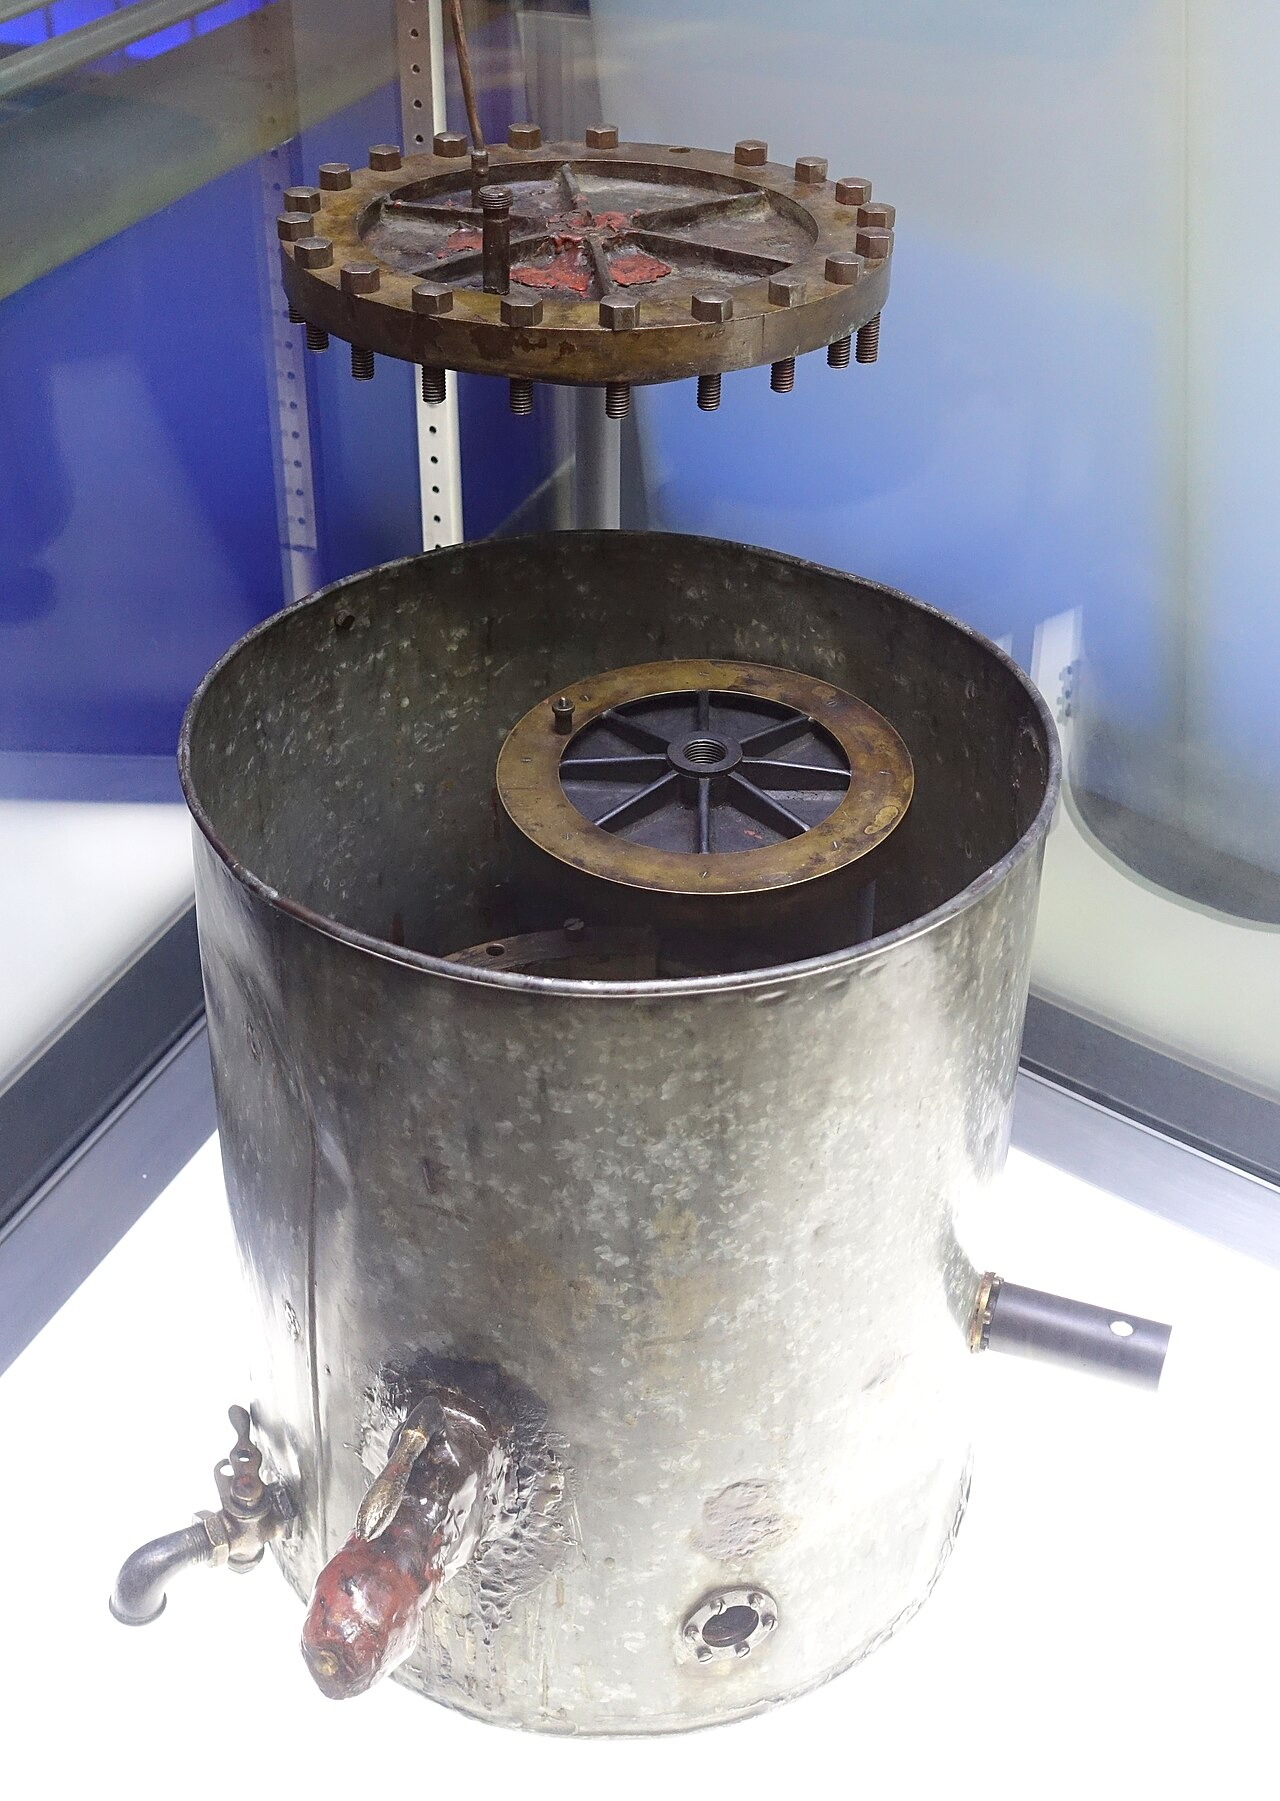
\includegraphics[width=0.36\linewidth]{images/book3/millikan-apparatus.jpg}

{\small جهاز قطرة الزيت عند ميليكان، نحو 1916 (متحف العلوم والصناعة في شيكاغو): وتحوي الحجرة النحاسية الصفيحتين الأفقيتين اللتين كانت القطرات تُرقَب بينهما.}
\end{omfigure}

\section{مسألة: قطرة زيت ميليكان}

\begin{problem}[{مسألة نهاية الأسبوع --- وزن شحنة الإلكترون
بقطرة زيت: ستوكس، والمكثف المستوي، وجدول من الأعداد
تأبى أن تكون إلا مضاعفات لعدد واحد}]
\label{pb:b1:potential-capacitors:1}
تُرشّ قطرات زيت بين صفيحتين أفقيتين تفترقان $d = \qty{16}{mm}$
وقطر كلٍّ منهما \qty{20}{cm}، وتُرقَب \omterm{def:b1:optical-instruments:microscope}{بمجهر}.
المعطيات: كثافة الزيت $\rho = \qty{900}{kg/m^3}$، وكثافة الهواء
\qty{1.2}{kg/m^3}، ولزوجة الهواء $\eta = \qty{1.8e-5}{Pa.s}$، و $g =
\qty{9.8}{m/s^2}$، و $\varepsilon_0 = \qty{8.85e-12}{F/m}$. وكرة صغيرة
نصف قطرها $r$ تتحرك بالسرعة $v$ في الهواء تحسّ بجرّ ستوكس $6\pi\eta rv$.

\medskip
\noindent\textbf{الجزء I --- القطرة الساقطة.}
\begin{enumerate}
  \item القوى المؤثرة في قطرة تسقط بلا توتر مطبَّق؛ وبيّن أنها
        تبلغ \omterm{prop:b1:newton-dynamics:terminal}{سرعة حدية} $v_1 = 2\rho gr^2/9\eta$ (بإهمال
        دافعة الهواء --- وبرّر ذلك).
  \item قطرة تسقط \qty{1.0}{mm} في \qty{10}{s}: أوجد نصف قطرها وكتلتها.
  \item \omterm{def:b1:transient-regimes:firstorder}{ثابت الزمن} للاقتراب من $v_1$؛ والمسافة المقطوعة
        في أثنائه. وهل تُرى القطرة متسارعة يومًا؟
  \item عدد رينولدز $\rho_{\text{الهواء}}v_1r/\eta$ للحركة: فهل
        قانون ستوكس مشروع؟
  \item ولماذا يجب أن تكون القطرات بهذا الصغر؟ (قارن الثقل بالقوة
        الكهربائية على \omterm{def:b1:electrostatics-gauss:charge}{شحنة أولية} واحدة في مجال قدره
        \qty{3e5}{V/m}.)
  \item تُرى القطرة ترتجف قليلًا حول متوسط سقوطها: فما هذا،
        ولماذا يحدّ من الدقة؟
\end{enumerate}

\medskip
\noindent\textbf{الجزء II --- المجال.}
يُطبَّق توتر $U$، والصفيحة العليا موجبة.
\begin{enumerate}[resume]
  \item المجال بين الصفيحتين من أجل $U = \qty{5.0}{kV}$؛ ولماذا هو
        منتظم، وما الأسطح المتساوية الكمون؟
  \item \omterm{def:b1:potential-capacitors:capacitance}{سعة} الصفيحتين، والشحنة عليهما عند \qty{5.0}{kV}، و
        الطاقة المخزونة.
  \item تُبقى قطرة السؤال~2 ساكنة من أجل $U_0 = \qty{1080}{V}$:
        أوجد إشارة شحنتها وقيمتها، بالكولوم وبمضاعفات $e$.
  \item ومع $U = \qty{5.0}{kV}$ تصعد القطرة نفسها بالسرعة $v_2$: بيّن أن
        $q = 6\pi\eta r(v_1 + v_2)d/U$ واحسب $v_2$.
  \item ولماذا يكون توقيت صعود وسقوط خيرًا من تصيّد توتر
        التوازن؟
  \item طاقة وضع شحنة القطرة بين الصفيحتين عند
        \qty{5}{kV}، والطاقة التي يبددها الجرّ في صعود قدره
        \qty{1}{cm}.
\end{enumerate}

\medskip
\noindent\textbf{الجزء III --- جدول الشحن.}
وبتعريض القطرة نفسها لمنبع ضعيف من الأشعة السينية بين القياسات،
تتغير شحنتها؛ وتعطي القياسات المتتالية (بوحدة $10^{-19}$~كولوم):
$4.80$ و $8.01$ و $6.42$ و $3.19$ و $9.63$.
\begin{enumerate}[resume]
  \item بيّن أن الخمسة كلها قريبة من مضاعفات صحيحة لمقدار
        واحد، وأعطِ الأعداد الصحيحة.
  \item أفضل تقدير \omterm{def:b1:electrostatics-gauss:charge}{للشحنة الأولية} من القيم الخمس؛
        \omterm{def:b1:units-dimensions:uncertainty}{والارتياب المعياري} للمتوسط (\cref{ch:b1:units-dimensions}).
  \item ولماذا تتغير الشحنة بأعداد صحيحة من $e$ بين
        القياسات؟
  \item بيّن أنه في هذه الطريقة يكون $q \propto \eta^{3/2}$: فبكم يزيح
        خطأ قدره $1\%$ في اللزوجة قيمةَ $e$؟ (وكانت قيمة ميليكان الأصلية
        أدنى بنسبة $0.6\%$، لهذا السبب بالذات.)
  \item تحمل الكواركات $\pm e/3$ و $\pm 2e/3$: فلماذا لم تُظهر قطرة زيت قط
        ثلث $e$؟
  \item ثابت فاراداي، وهو شحنة \omterm{def:b1:kinetic-theory:scales}{مول} من الإلكترونات، يساوي
        $F = \qty{96485}{C/mol}$: استنتج عدد أفوغادرو.
  \item وكان طومسون قد قاس للإلكترون $e/m_e = \qty{1.76e11}{C/kg}$:
        فاستنتج: استنتج كتلته، وقارنها بذرة هيدروجين
        (\qty{1.67e-27}{kg}).
\end{enumerate}

\medskip
\noindent\textbf{الجزء IV --- الجهاز، بلغة الكمون.}
\begin{enumerate}[resume]
  \item ارسم الأسطح المتساوية الكمون \omterm{def:b1:electrostatics-gauss:field}{وخطوط المجال} بين الصفيحتين،
        بما في ذلك الانتشار عند الحواف؛ وبرّر إهماله.
  \item قطرة مشحونة موجبةً على ارتفاع $z$ فوق الصفيحة السفلى
        (وهي عند \qty{0}{V}): أوجد طاقة الوضع بدلالة $z$؛ وطاقة الوضع
        الكلية بما فيها الثقالة؛ والشرط على $U$ من أجل النقطة الساكنة.
  \item قارن طاقة شحنة القطرة (السؤال~12) مع
        الطاقة المخزونة في \omterm{def:b1:potential-capacitors:capacitance}{المكثف}: فهل تضطرب القطرةُ المجالَ؟
  \item ويُعكس التوتر (فتصير الصفيحة السفلى موجبة) مع
        $U = \qty{5.0}{kV}$: فماذا تفعل قطرة السؤال~9، وبأيّ
        سرعة؟
  \item حبة غبار كتلتها \qty{1}{\micro g} تحمل $10^4e$ في المجال
        نفسه: أوجد نسبة القوة الكهربائية إلى الثقل؛ ولماذا لا يمكن رفع مثل
        هذه الحبات، ولماذا اختار ميليكان رذاذ الزيت.
  \item لخّص: ما الذي قيس (ثلاث مرات)، وما الذي استُنتج،
        وبأيّ ارتياب، وأيّ ثابتين تبعا ذلك.
\end{enumerate}
\end{problem}
